This section presents IJM's deployment topology, the~four-phase
scheduling pipeline that drives every dispatch decision, the~worker
execution lifecycle that~runs and~stops each container, the~job state
machine, the~persistent state held in~PostgreSQL, and~the~concurrency
invariants that keep the~control plane consistent under racing API
calls and~worker notifications.  Table~\ref{tab:components} catalogues
every component referenced in~the~rest of~the~chapter.

\begin{table}[H]
\centering\small
\begin{tabularx}{\textwidth}{@{}l l X@{}}
\toprule
\textbf{Component} & \textbf{Process} & \textbf{Responsibility} \\
\midrule
API                       & \texttt{ijm-api} (FastAPI) & HTTP frontend; hosts the~scheduling and~dispatch loops \\
\texttt{ProfilingScheduler} & in-API & Picks the~next unmeasured \texttt{(node, GPU-count)} cell for~profile-owing rows \\
\texttt{JobDispatcher}      & in-API & Acquires the~destination's \texttt{NodeSlots} permit, then~POSTs \texttt{/jobs/\{id\}/run} to~the~target worker \\
\texttt{NodeSlots}          & in-API & Per-node semaphore tracking GPU permits; reconciled with the~DB by~a~periodic drift heartbeat \\
\texttt{ClusterManager}     & in-API & Loads \texttt{nodes\_config.json} and~exposes node and~GPU resources \\
Optimizer client          & in-API & Packages the~GPUspb request, parses the~returned assignments and~preempts \\
Worker                    & \texttt{ijm-worker} (FastAPI) & Owns the~local Docker daemon; performs atomic claim, runs the~container, emits slot-freed notifications \\
PostgreSQL                & DB & Source of~truth for~job rows and~profile measurements \\
GPUspb optimiser          & external HTTP & Cost-aware standard-run placement (reached via~\texttt{OPTIMIZER\_URL}) \\
SPA                       & static (Vite) & Operator UI; polls the~API every 3--5~s \\
\bottomrule
\end{tabularx}
\caption{IJM components and~their responsibilities.}\label{tab:components}
\end{table}

\section{Deployment topology}

IJM runs as~a~small distributed system.  The~FastAPI \emph{API}~--- which
also hosts the~\texttt{ProfilingScheduler}, the~\texttt{JobDispatcher},
the~\texttt{NodeSlots} semaphores, and~the~optimiser client~--- runs on
the~operator's machine.  A~lightweight FastAPI \emph{worker} runs on
every GPU node and~owns the~local Docker daemon.  PostgreSQL runs on
one of~the~GPU nodes.

Communication is~plain HTTP over SSH tunnels.  Every worker is~reached
from the~API at~a~stable \texttt{http://localhost:800x} alias regardless
of~its physical location, so the~same scheduler code drives a~laptop
talking to~a~remote cluster and~a~single-host development setup.
An~optional GPUspb \emph{optimiser} HTTP service is~reached the~same
way.

\begin{figure}[H]
\centering
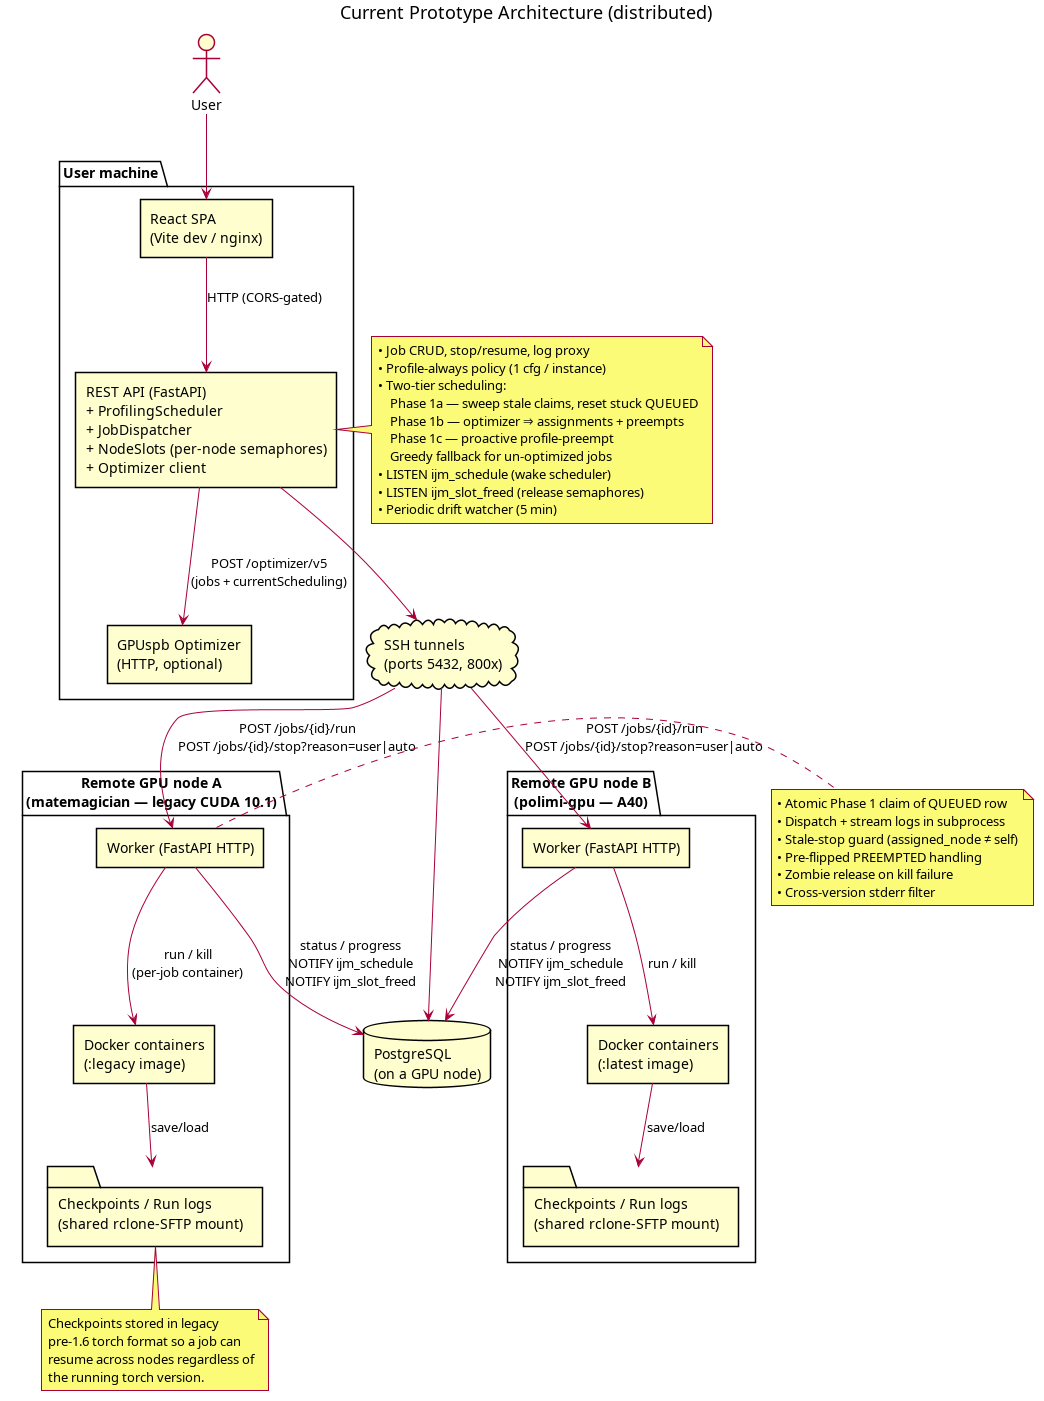
\includegraphics[width=\textwidth]{Images/CurrentPrototype.png}
\caption{Distributed prototype.  The~SPA, API, and~optimiser run on
the~operator's machine; workers and~Docker run on~each GPU node;
PostgreSQL runs on~a~GPU~node.  A~shared rclone-over-SFTP mount makes
checkpoints written by~one node visible from the~other.}
\label{fig:prototype}
\end{figure}

Single-process \texttt{docker compose} on~the~operator's machine is
supported for~development but is~not the~deployment target: any tradeoff
between local-dev simplicity and~distributed correctness resolves toward
the~distributed topology.

\section{Scheduling pipeline}\label{sec:sched-pipeline}

The pipeline is~shaped by~a~single governing assumption: \emph{profiling
is~always worth its cost}.  A~deep-learning job runs for~hours, whereas
profiling one GPU~configuration takes minutes; leaving a~configuration
unmeasured risks overlooking the~placement that~would have saved hours
of~computation, or~missing a~hard deadline.  The~scheduler therefore
treats profiling as~privileged work that~may preempt running jobs,
rather than as~best-effort measurement deferred until the~cluster falls
idle.  How~aggressively the~system profiles is~a~tunable policy:
\texttt{PROFILING\_CONFIGS\_PER\_JOB} (default~2) sets how~many
configurations each instance must measure before it~is~handed to~the
cost-aware optimiser for~standard placement.

A~single scheduling pass~--- \texttt{\_schedule\_waiting\_jobs} in
\texttt{app.py}~--- handles every dispatch decision.  It is~invoked
whenever a~job is~submitted, a~profiling run finishes, or~a~slot is
freed.  A~60-minute watchdog (\texttt{\_queue\_watcher}) serves as~a
safety net for~missed notifications, not as~the~main wake source.
Wake-ups are coalesced through a~single
\texttt{asyncio.Event} and~rate-limited to~at~most one pass every
five~seconds, so the~cluster has time to~apply the~previous plan before
the~next one is~computed.

The pass runs four phases, all guarded by~a~single
\texttt{schedule\_lock} except the~optimiser's HTTP call (phase~2),
which is~made outside the~lock so its timeout cannot stall concurrent
scheduler work:

\begin{enumerate}[leftmargin=*,itemsep=2pt,topsep=4pt]
  \item \textbf{Reset stuck assignments.}
    Reset \texttt{QUEUED} rows whose \texttt{assigned\_node} was set
    $\geq 30$~s ago without the~worker advancing them, so a~later phase
    can re-place the~row.
  \item \textbf{Optimiser pass.}
    Call the~optimiser outside the~lock (to~accommodate its 30~s HTTP
    timeout) and~apply its assignments through a~conditional
    \texttt{UPDATE \ldots WHERE assigned\_node IS NULL}, collecting the
    optimiser's preempt list.  The~optimiser only ever scores rows with
    \texttt{is\_profiling\_run = FALSE}~--- rows still owing a~profile
    run are invisible to~it.
  \item \textbf{Profile placement.}
    For~\texttt{QUEUED} rows that still owe a~profile run, the
    \texttt{ProfilingScheduler} atomically reserves the~instance's
    outstanding unmeasured \texttt{(node, GPU-count)} cells~--- up to~its
    \texttt{PROFILING\_CONFIGS\_PER\_JOB} budget (default~2)~--- and
    dispatches one of~them this pass, choosing the~node by~best fit
    on~remaining capacity; the~rest follow on~later passes as~slots
    free.  This is~the~mechanism behind the~\emph{profile-always}
    policy: an~instance must complete all~its profile runs before
    it~becomes a~candidate for~the optimiser-driven standard placement
    above.
  \item \textbf{Profile-preempt.}
    If~a~profile-owing row still has~no~slot after the~placement pass,
    find the~cheapest set of~low-priority \texttt{RUNNING} jobs whose
    eviction would free enough GPUs for~the~next unmeasured
    configuration.
\end{enumerate}

Once the~lock is~released, the~plan is~executed asynchronously: each
preempt and~each dispatch runs as~an~independent task, so a~slow stop
on~one node never delays placements on~another.  Before launching a~job,
the~dispatcher must acquire a~permit from the~destination node's
\texttt{NodeSlots} semaphore, whose count is~that node's GPU~capacity;
the~permit is~what bounds the~number of~concurrent jobs per~node and
arbitrates between tasks competing for~the~last free slot.

Permits are released asynchronously, because a~job's GPUs are not free
the~instant the~API decides to~stop it~--- only once the~worker has
killed the~container, drained its logs, and~written a~checkpoint.  The
worker therefore signals each release, and~the~API returns the~permit
at~that moment, keeping its in-memory count in~step with actual
occupancy.  Each release also records \emph{why} it~happened, because
the~cause determines whether the~scheduler should re-plan.  A~release
triggered by~an~event outside the~current plan~--- a~job finishing
on~its own, an~operator stopping a~job, or~the~cleanup of~an~orphaned
container~--- frees capacity the~optimiser did not foresee, and~so wakes
a~fresh scheduling pass.  A~release caused by~the~scheduler's \emph{own}
in-flight preempt is~the~one exception: the~plan that~issued the~preempt
already contains the~dispatch that~will reclaim the~freed slot, so
re-running the~optimiser at~that point would let it~rewrite a~plan it~is
still executing.  Only that case suppresses the~re-plan, and~doing so
is~safe because independent watchdogs~--- a~drift heartbeat, the
stuck-dispatch reaper, and~a~periodic queue watcher~--- re-wake the
scheduler if~a~planned dispatch ever fails to~land.

Figure~\ref{fig:seq-submit} shows the~submission path,
Figure~\ref{fig:seq-profiling-loop} the~cross-instance profile cycle,
Figure~\ref{fig:seq-optimizer-cycle} an~optimiser-driven preempt and
migrate round, and~Figure~\ref{fig:seq-standard-run} the~standard run.

\begin{figure}[H]
\centering
\footnotesize
\setlength{\unitlength}{0.7cm}
\resizebox{\textwidth}{!}{%
\begin{sequencediagram}
  \newthread{user}{User}
  \newinst[1.5]{api}{API}
  \newinst[1.5]{sched}{Scheduler}
  \newinst[1.5]{opt}{Optimizer}
  \newinst[1.5]{db}{PostgreSQL}
  \newinst[1.5]{worker}{Worker}

  \begin{call}{user}{\textsc{post} /jobs \{job\_id, dockerImage, \ldots\}}{api}{instance\_id}
    \begin{call}{api}{INSERT INTO jobs (status=QUEUED)}{db}{}
    \end{call}
    \begin{messcall}{api}{NOTIFY ijm\_schedule}{db}
    \end{messcall}
  \end{call}
  \begin{sdblock}{schedule pass}{coalesced, $\geq 5$s apart}
    \begin{call}{sched}{sweep stale claims; reset stuck QUEUED}{db}{}
    \end{call}
    \begin{call}{sched}{optimize(active jobs, currentScheduling)}{opt}{assignments, preempts}
    \end{call}
    \begin{call}{sched}{UPDATE assigned\_node WHERE NULL}{db}{}
    \end{call}
    \begin{callself}{sched}{profile-placement + profile-preempt scan}{}
    \end{callself}
    \begin{messcall}{sched}{dispatch\_with\_slot $\rightarrow$ acquire permit $\rightarrow$ POST /run}{worker}
    \end{messcall}
  \end{sdblock}
\end{sequencediagram}}
\caption{Submission and~scheduling.  The~API writes the~row and~notifies
the~scheduler; placement is~decided by~the~next pass.  The~optimiser
call sits outside the~schedule lock so its 30~s HTTP timeout cannot
block other passes.}
\label{fig:seq-submit}
\end{figure}

\begin{figure}[H]
\centering
\footnotesize
\setlength{\unitlength}{0.7cm}
\resizebox{\textwidth}{!}{%
\begin{sequencediagram}
  \newthread{worker}{Worker}
  \newinst[1.5]{docker}{Docker}
  \newinst[1.5]{sched}{Scheduler}
  \newinst[1.5]{db}{PostgreSQL}

  \begin{call}{worker}{atomic claim: UPDATE \ldots status=PROFILING}{db}{ok}
  \end{call}
  \begin{call}{worker}{docker run (profile container, isolated ckpt dir)}{docker}{exit code}
  \end{call}
  \begin{callself}{worker}{mean per-epoch duration (warmup epoch excluded)}{}
  \end{callself}
  \begin{call}{worker}{UPDATE profiling\_results SET duration\_seconds}{db}{}
  \end{call}
  \begin{call}{worker}{UPDATE jobs SET status=QUEUED, is\_profiling\_run=still\_owes}{db}{}
  \end{call}
  \begin{messcall}{worker}{NOTIFY ijm\_schedule}{db}
  \end{messcall}
  \begin{sdblock}{next scheduling pass}{}
    \begin{callself}{sched}{place this row as standard run, or pick next config to profile}{}
    \end{callself}
  \end{sdblock}
\end{sequencediagram}}
\caption{Profiling cycle.  Profile measurements are keyed by~the
(job-type, GPU-config) pair and~shared across submissions of~the~same
type.  Each instance profiles up~to~\texttt{PROFILING\_CONFIGS\_PER\_JOB}
(default~2) configurations before it~becomes a~standard-run candidate;
the~per-instance claim row guards against duplicate measurements.  The
worker records the~result and~re-queues the~row in~a~single transaction
(\texttt{worker/profiling.py:handle\_complete}).}
\label{fig:seq-profiling-loop}
\end{figure}

\begin{figure}[H]
\centering
\footnotesize
\setlength{\unitlength}{0.7cm}
\resizebox{\textwidth}{!}{%
\begin{sequencediagram}
  \newthread{sched}{Scheduler}
  \newinst[1.5]{opt}{Optimizer}
  \newinst[1.5]{db}{PostgreSQL}
  \newinst[1.5]{victim}{Worker (victim)}
  \newinst[1.5]{target}{Worker (target)}

  \begin{call}{sched}{POST /optimizer/v5 \{jobs, nodes, currentScheduling\}}{opt}{assignments + preempts}
  \end{call}
  \begin{callself}{sched}{stash pending\_migrates (in-memory)}{}
  \end{callself}
  \begin{messcall}{sched}{POST /stop?reason=auto}{victim}
  \end{messcall}
  \begin{call}{victim}{kill container, drain run task}{db}{}
    \begin{call}{victim}{UPDATE jobs SET status=QUEUED, assigned\_node=NULL}{db}{}
    \end{call}
    \begin{messcall}{victim}{NOTIFY ijm\_slot\_freed "node:n:auto\_preempt"}{db}
    \end{messcall}
  \end{call}
  \begin{callself}{sched}{release NodeSlots permit on LISTEN}{}
  \end{callself}
  \begin{call}{sched}{apply pending migrate on slot-freed LISTEN (\textsc{where} assigned\_node \textsc{is null})}{db}{}
  \end{call}
  \begin{messcall}{sched}{dispatch\_with\_slot $\rightarrow$ POST /run}{target}
  \end{messcall}
\end{sequencediagram}}
\caption{Optimiser-driven preempt and~migrate.  The~API trusts the
GPUspb plan: any job in~\texttt{currentScheduling} that the~optimiser
drops or~moves is~preempted with~\texttt{reason=auto}, clearing its
assignment.  Because an~\texttt{auto\_preempt} release deliberately does
\emph{not} wake a~fresh optimiser pass, a~moved job's new placement is
stashed in~\texttt{state.pending\_migrates} and~re-applied by~the~slot
listener (conditional \texttt{UPDATE \ldots WHERE assigned\_node IS
NULL}) once the~source \texttt{/stop} has drained the~row to
\textsc{queued}.}
\label{fig:seq-optimizer-cycle}
\end{figure}

\begin{figure}[H]
\centering
\footnotesize
\setlength{\unitlength}{0.7cm}
\resizebox{\textwidth}{!}{%
\begin{sequencediagram}
  \newthread{worker}{Worker}
  \newinst[1.5]{docker}{Docker}
  \newinst[1.5]{sched}{Scheduler}
  \newinst[1.5]{db}{PostgreSQL}

  \begin{call}{worker}{atomic claim: UPDATE \ldots status=RUNNING}{db}{ok}
  \end{call}
  \begin{call}{worker}{docker run (training container)}{docker}{exit code}
  \end{call}
  \begin{call}{worker}{UPDATE jobs SET SUCCEEDED/FAILED}{db}{}
  \end{call}
  \begin{messcall}{worker}{NOTIFY ijm\_slot\_freed "node:n:terminal"}{db}
  \end{messcall}
  \begin{sdblock}{next scheduling pass}{}
    \begin{callself}{sched}{place a waiting job on the freed slot}{}
    \end{callself}
  \end{sdblock}
\end{sequencediagram}}
\caption{Standard run.  The~worker performs an~atomic
conditional \texttt{UPDATE \ldots WHERE status = ANY(RUNNABLE\_STATUSES)}
so concurrent stops or~duplicate dispatches cannot race a~row into
\texttt{RUNNING}.  On~exit the~worker fires a~single
\texttt{ijm\_slot\_freed} (reason~\texttt{terminal}) in~the~same
transaction as~the~status flip; the~slot listener releases the~permit
and~wakes the~scheduler, so the~terminal path needs no~separate
\texttt{ijm\_schedule}.}
\label{fig:seq-standard-run}
\end{figure}

\section{Worker execution lifecycle}\label{sec:worker-lifecycle}

The scheduling pass decides \emph{where} a~job runs; the~worker's run
task (\texttt{\_run\_job}) owns \emph{how} it~runs and~how it~stops.  The
task moves through four phases (Table~\ref{tab:worker-phases}), and~every
database transition is~a~conditional \texttt{UPDATE}, so a~racing
\texttt{/stop}, the~stuck-dispatch reaper, or~a~duplicate dispatch cannot
corrupt the~row.

\begin{table}[H]
\centering\small
\begin{tabularx}{\textwidth}{@{}l >{\raggedright\arraybackslash}X >{\raggedright\arraybackslash}X@{}}
\toprule
\textbf{Phase} & \textbf{Action} & \textbf{Invariant it~enforces} \\
\midrule
1.~Claim    & Atomic \texttt{UPDATE \ldots status=RUNNING/PROFILING WHERE status} $\in$ \textsc{runnable} \texttt{AND assigned\_node=self} & A~\texttt{/stop} or~reaper that~already moved the~row makes the~claim miss, so no~container starts for~a~re-placed row. \\
2.~Launch   & Pick distinct physical GPU indices, prepare the~per-job checkpoint/runs directories, \texttt{docker run} & Distinct indices stop two 1-GPU jobs both landing on~GPU~0; an~in-process placeholder is~set \emph{before} any~\texttt{await}, so a~\texttt{/stop} cannot slip into the~window before the~container exists. \\
3.~Stream   & Parse \texttt{Epoch x/y} from~container stdout; flush the~latest value through a~once-per-second background writer & The~progress \texttt{UPDATE} is~conditional on~a~matching \texttt{status} and~\texttt{container\_name}, so a~reassigned row no-ops it~and~stops the~stream.  Coalescing replaces a~per-epoch round-trip that~fell behind over the~SSH-tunnelled connection. \\
4.~Complete & Write the~terminal status and~fire one~\texttt{ijm\_slot\_freed}; or, if~the~row was~migrated or~already stopped, record only the~exit code & A~kill-induced exit~137 never clobbers the~new owner's \textsc{running}; a~failed run also drops its~outstanding profile claims so their~cells are~not~left reserved. \\
\bottomrule
\end{tabularx}
\caption{The~worker run task's four phases~--- distinct from~the
scheduling pass's four phases above: that pass plans, this~task
executes.}\label{tab:worker-phases}
\end{table}

A~\texttt{/stop} and~its target run task are~separate coroutines that~must
not~race.  The~handler tags the~row in~an~in-process \texttt{stopping}
map, waits for~the~run task to~publish its~container
(\texttt{dispatch\_ready}), kills it, and~only \emph{after} awaiting the
run task's full drain writes the~final status and~frees the~slot
(Figure~\ref{fig:seq-worker-stop}).  The~run task's own completion phase,
seeing the~\texttt{stopping} tag, records just the~exit code, so the~slot
is~freed exactly once.  The~same hazard across nodes is~closed on~the~API
side: \texttt{dispatch\_with\_slot} awaits any in-flight \texttt{/stop}
on~the~target node before posting \texttt{/run}, so a~migration's new
container never starts before the~evicted one's CUDA context has~released
its~GPU.

\begin{figure}[H]
\centering
\footnotesize
\setlength{\unitlength}{0.7cm}
\resizebox{\textwidth}{!}{%
\begin{sequencediagram}
  \newthread{api}{API}
  \newinst[1.6]{run}{Worker run task}
  \newinst[1.6]{dock}{Docker}
  \newinst[1.6]{stop}{Worker /stop}
  \newinst[1.6]{db}{PostgreSQL}

  \begin{call}{api}{POST /run}{run}{202}
  \end{call}
  \begin{call}{run}{Phase 1: atomic claim status=RUNNING}{db}{ok}
  \end{call}
  \begin{call}{run}{Phase 2: docker run; set dispatch\_ready}{dock}{}
  \end{call}
  \begin{callself}{run}{Phase 3: stream stdout, progress @ 1/s}{}
  \end{callself}
  \begin{messcall}{api}{POST /stop?reason=auto  (stopping := auto)}{stop}
  \end{messcall}
  \begin{callself}{stop}{await dispatch\_ready}{}
  \end{callself}
  \begin{call}{stop}{kill container}{dock}{}
  \end{call}
  \begin{sdblock}{/stop awaits the run-task drain, then persists once}{}
    \begin{messcall}{dock}{exit 137}{run}
    \end{messcall}
    \begin{callself}{run}{Phase 4: stopping set $\Rightarrow$ record exit\_code only}{}
    \end{callself}
    \begin{call}{stop}{\_persist\_stop: status=QUEUED, assigned\_node=NULL}{db}{}
    \end{call}
    \begin{messcall}{stop}{NOTIFY ijm\_slot\_freed "node:n:auto\_preempt"}{db}
    \end{messcall}
  \end{sdblock}
\end{sequencediagram}}
\caption{Worker execution and~a~scheduler stop.  The~run task and~the
concurrent \texttt{/stop} synchronise through the~in-process
\texttt{dispatch\_ready} and~\texttt{stopping} maps plus a~drain await, so
the~slot is~freed exactly once and~by~exactly one path.  A
\texttt{reason=auto} stop returns the~row to~\textsc{queued} with~its
assignment cleared (a~\texttt{reason=user} stop lands on~\textsc{preempted}
instead); the~resulting \texttt{auto\_preempt} notify is~the~one the~slot
listener swallows (\S\ref{sec:sched-pipeline}).}
\label{fig:seq-worker-stop}
\end{figure}

\section{State machine}

Table~\ref{tab:state-machine} lists every transition a~job row can take.
All transitions are driven by~atomic conditional \texttt{UPDATE}s, so
concurrent stop, dispatch, and~completion paths cannot clobber each
other's work.

\begin{table}[H]
\centering\small
\begin{tabularx}{\textwidth}{@{}l l X@{}}
\toprule
\textbf{From} & \textbf{To} & \textbf{Trigger} \\
\midrule
\textsc{queued}     & \textsc{profiling} / \textsc{running} & Worker Phase~1 atomic claim \\
\textsc{profiling}  & \textsc{queued}     & Profile run finished; \texttt{is\_profiling\_run} flips to~\texttt{false} \\
\textsc{profiling}  & \textsc{failed}     & Profile container exited non-zero \\
\textsc{running}    & \textsc{succeeded} / \textsc{failed} & Container exit \\
\textsc{running}    & \textsc{preempted}  & User \texttt{POST /jobs/\{id\}/stop?reason=user} \\
\textsc{running}    & \textsc{queued}     & Scheduler preempt (\texttt{reason=auto}): clears \texttt{assigned\_node} for~the~next pass \\
\textsc{preempted} / \textsc{failed} & \textsc{queued} & \texttt{POST /jobs/\{id\}/resume} \\
\bottomrule
\end{tabularx}
\caption{Job state transitions.}\label{tab:state-machine}
\end{table}

Two distinct stop reasons separate \emph{user-initiated} preemption from
\emph{scheduler-initiated} preemption.  A~user stop is~sticky:
\textsc{preempted} stays put until the~user explicitly resumes.  A
scheduler stop returns the~row to~\textsc{queued} with~a~cleared
assignment, so the~next pass can place it~elsewhere automatically.  The
worker enforces this distinction and~ignores stale \texttt{/stop} calls
aimed at~a~row that has~since been re-assigned to~another node.

\section{Persistent state}\label{sec:persistent-state}

Two PostgreSQL tables hold every fact the~scheduler reads or~writes;
both are created idempotently on~startup from~\texttt{backend/schema.sql}.

\begin{lstlisting}[language=SQL, numbers=none]
CREATE TABLE jobs (
    id                  TEXT PRIMARY KEY,
    job_id              TEXT NOT NULL,
    image               TEXT NOT NULL,
    command             JSONB NOT NULL,
    script_path         TEXT,
    directory_to_mount  TEXT,
    status              TEXT NOT NULL,
    created_at          TIMESTAMPTZ NOT NULL,
    updated_at          TIMESTAMPTZ NOT NULL,
    container_name      TEXT,
    exit_code           INT,
    progress            TEXT,
    priority            INT DEFAULT 3,
    deadline            TIMESTAMPTZ,
    batch_size          INT,
    epochs_total        INT,
    profiling_epochs_no INT,
    assigned_node       TEXT,
    assigned_gpu_config JSONB,
    is_profiling_run    BOOLEAN DEFAULT FALSE
);

CREATE TABLE profiling_results (
    id               TEXT PRIMARY KEY,
    job_id           TEXT NOT NULL,
    instance_id      TEXT,
    gpu_config       JSONB NOT NULL,
    node_id          TEXT NOT NULL,
    duration_seconds FLOAT,
    created_at       TIMESTAMPTZ NOT NULL
);
\end{lstlisting}

Two columns of~\texttt{jobs} are load-bearing for~the~scheduling pass
above: \texttt{assigned\_node} is~the~target the~optimiser pass writes
under \texttt{WHERE assigned\_node IS NULL}, and~\texttt{is\_profiling\_run}
is~the~flag that makes a~row invisible to~the~optimiser (phase~2) and
visible to~the~\texttt{ProfilingScheduler} (phases~3--4).

A~unique index on~\texttt{(job\_id, gpu\_config)} makes the
cross-instance profile claim atomic.  Profile measurements are keyed
by~the~\emph{job type} (\texttt{job\_id}) and~the~GPU configuration, so
two concurrent submissions of~the~same type race to~own each unmeasured
cell; the~loser's INSERT trips the~unique constraint and~the~winner's
measurement is~shared by~every subsequent instance of~that type.

\section{Concurrency invariants}

The control plane relies on~three invariants, each defended in~code.

\textbf{No GPU oversubscription.}  Every dispatch goes through
\texttt{NodeSlots.acquire(node\_id,\,n\_gpus)}.  On~startup the
semaphores are reconciled from the~database: only rows in~\textsc{running}
or~\textsc{profiling} pre-acquire their permits, since a~\textsc{queued}
row with~an~assigned node has~no~live container yet (its dispatch task
acquires the~permit just before posting \texttt{/run}).  A~periodic drift
watcher recomputes the
authoritative count at~the~\texttt{IJM\_DRIFT\_HEARTBEAT\_S} cadence
(default 15~s) and~corrects any divergence.

\textbf{No duplicate containers per row.}  Both the~worker (Phase~1
claim, \texttt{running\_jobs[job\_id]} check) and~the~API
(\texttt{dispatch\_tasks[instance\_id]} deduplication) refuse a~second
concurrent dispatch for~the~same instance.  The~reaper that resets stuck
\textsc{queued} rows cancels any live dispatch task instead of
double-releasing its permit.

\textbf{Profiling is~sacred.}  Auto-preempt
(\texttt{\_preempt\_and\_release}) refuses to~act on
\texttt{is\_profiling\_run=TRUE}, and~profile-preempt (phase~4) filters
victims by~\texttt{status='RUNNING'} only.  Only an~explicit user stop
can cancel an~in-flight measurement.

\section{Stoppable, resumable, cross-node training}\label{sec:checkpoints}

A~job is~\emph{stoppable} because the~trainer persists its~state after
every epoch, and~\emph{resumable} because every (re)start loads that
state.  \texttt{BaseTrainer.train} writes \texttt{latest.pt} at~the~end
of~each epoch through a~temp-file-and-\texttt{rename}, so the~on-disk
checkpoint is~always a~whole epoch, never a~half-written file.  Stopping
a~job is~therefore just killing its~container
(\S\ref{sec:worker-lifecycle}): the~in-progress epoch is~discarded,
every completed epoch is~durable.  The~next dispatch~--- on~the~same node
or~another~--- reconstructs the~trainer, which loads \texttt{latest.pt},
restores the~model, optimiser, and~\texttt{current\_epoch}, and~continues
the~loop (Figure~\ref{fig:seq-resume}).  No~scheduler state mirrors
training progress; the~checkpoint file is~the~single source of~truth for
how far a~job has~run.

\begin{figure}[H]
\centering
\footnotesize
\setlength{\unitlength}{0.7cm}
\resizebox{0.85\textwidth}{!}{%
\begin{sequencediagram}
  \newthread{r1}{Trainer run --- node A}
  \newinst[2.4]{fs}{latest.pt (shared FS)}
  \newinst[2.4]{r2}{Trainer run --- node B}

  \begin{callself}{r1}{epoch $k$: train + evaluate}{}
  \end{callself}
  \begin{call}{r1}{atomic save (temp file $\rightarrow$ rename)}{fs}{}
  \end{call}
  \begin{callself}{r1}{epoch $k{+}1$: training\ldots\ container killed}{}
  \end{callself}
  \begin{call}{r2}{load $\Rightarrow$ epoch $k$, model + optimiser (strict=False)}{fs}{state}
  \end{call}
  \begin{callself}{r2}{resume from epoch $k{+}1$}{}
  \end{callself}
\end{sequencediagram}}
\caption{Stop and~resume.  The~trainer checkpoints after each epoch with
a~temp-file-and-\texttt{rename}, so \texttt{latest.pt} is~never
half-written.  A~stop kills the~container mid-epoch; the~next run~--- here
on~a~different node, possibly a~different torch version~--- loads
\texttt{latest.pt} and~continues.  Only the~interrupted epoch~$k{+}1$
is~recomputed.}
\label{fig:seq-resume}
\end{figure}

Two GPU generations coexist, so a~resume must survive a~change of~torch
version mid-job.  The~\texttt{matemagician} node is~pinned to~driver~418.x
(CUDA~10.1 max), so it~runs a~separate \texttt{:legacy} image built
on~PyTorch~1.5.1 and~Python~3.7; the~remaining nodes run the~default
\texttt{:latest} image on~PyTorch~2.6 and~CUDA~12.4.  Both images write
the~checkpoint in~the~legacy pre-1.6 \texttt{torch.save} format, and~the
load is~deliberately lenient: \texttt{strict=False} tolerates state-dict
key differences between versions, and~a~failed optimiser-state load
restarts Adam from~scratch rather than aborting the~resume~--- the~model
weights are~what matter, and~a~few epochs of~optimiser warmup are
invisible at~scenario timescales.  This is~what lets \texttt{cnn\_big}
migrate between a~modern A40 and~a~legacy P600 without losing progress.

The shared \texttt{data/} directory is~mounted on~every node via~rclone
over SFTP.  It~contains:

\begin{itemize}
  \item \texttt{data/checkpoints/\{job\_id\}/}~--- per-job checkpoints,
        mounted into the~container at~\texttt{/checkpoints};
  \item \texttt{data/runs/\{job\_id\}/}~--- captured stdout
        (\texttt{output.log}) and~TensorBoard artifacts, mounted at
        \texttt{/runs};
  \item \texttt{data/shared/data/}~--- read-only dataset cache (MNIST,
        CIFAR-10), mounted at~\texttt{/runs/data}.
\end{itemize}

Two worker-side environment variables let the~same
\texttt{nodes\_config.json} drive heterogeneous nodes.
\texttt{WORKER\_GPU\_MODE} selects how Docker exposes GPUs to~the
training container: \texttt{runtime} for~the~standard NVIDIA runtime,
\texttt{cdi} for~the~rootless daemon on~\texttt{polimi-gpu}, and
\texttt{none} for~a~CPU-only sandbox.  \texttt{IMAGE\_TAG\_OVERRIDE}
rewrites the~image tag, which is~how \texttt{matemagician} swaps
\texttt{:latest} for~\texttt{:legacy}.
